\documentclass{article}

\usepackage{booktabs}
\usepackage{fancyhdr}
\usepackage{float}
\usepackage{graphicx}
\usepackage{helvet}
\usepackage{hyperref}
\usepackage{tabularx}
\usepackage{xcolor}
\usepackage{wasysym}
\usepackage{color, colortbl}

\usepackage{listings}
\usepackage{tikz}
\usepackage{tikz-dimline}

\usetikzlibrary{shapes,arrows,positioning}

\usepackage{makeidx}         % allows index generation
\makeindex

\lstset{frame=tblr,
  rulecolor=\color{lightgray},
  language=Java,
  aboveskip=5mm,
  belowskip=5mm,
  showstringspaces=false,
  columns=flexible,
  basicstyle=\linespread{1.0}\small\ttfamily,
  numbers=none,
  % numberstyle=\tiny\color{gray},
  % keywordstyle=\color{blue},
  % commentstyle=\color{dkgreen},
  % stringstyle=\color{mauve},
  breaklines=true,
  breakatwhitespace=true,
  tabsize=3
}

\usepackage{framed}     % These needed for the code formatter
\usepackage{color}
\usepackage{fancyvrb}

% Use helvetica (sans) by default
\renewcommand{\familydefault}{\sfdefault}

% Greenish links
\hypersetup{
  colorlinks=true,
  linkcolor=blue!50!red,
  urlcolor=blue!50!red
}

\setlength{\headheight}{40pt}
\setlength{\headsep}{0.2in}

\pagestyle{fancy}
\lhead{
\includegraphics[width=0.2\textwidth]{img/logo}}
\chead{Gameduino 3X Dazzler}
\rhead{\thepage}
\cfoot{\textcopyright \the\year \ \ Excamera Labs}
\renewcommand{\headrulewidth}{0.5pt}
\renewcommand{\footrulewidth}{0.5pt}

\usepackage{array}
\newcolumntype{L}[1]{>{\raggedright\let\newline\\\arraybackslash\hspace{0pt}}m{#1}}
\newcolumntype{C}[1]{>{\centering\let\newline\\\arraybackslash\hspace{0pt}}m{#1}}
\newcolumntype{R}[1]{>{\raggedleft\let\newline\\\arraybackslash\hspace{0pt}}m{#1}}

\usepackage{setspace}

\newcommand{\device}{Gameduino 3X Dazzler}
\newcommand{\dev}{Dazzler}

\newcommand{\heavyline}{\specialrule{1pt}{1pt}{1pt}}
\newcommand{\png}[1]{
\begin{figure}[H]
\begin{center}
\includegraphics[width=0.75\textwidth]{#1}
\end{center}
\end{figure}
}
\newcommand{\pngw}[2]{
\begin{figure}[H]
\begin{center}
\includegraphics[width=#2\textwidth]{#1}
\end{center}
\end{figure}
}

\newcommand{\mach}[1]{\texttt{\textbf{#1}}}
\newcommand{\gap}{\vspace{10pt}}


\makeatletter
\def\PY@reset{\let\PY@it=\relax \let\PY@bf=\relax%
    \let\PY@ul=\relax \let\PY@tc=\relax%
    \let\PY@bc=\relax \let\PY@ff=\relax}
\def\PY@tok#1{\csname PY@tok@#1\endcsname}
\def\PY@toks#1+{\ifx\relax#1\empty\else%
    \PY@tok{#1}\expandafter\PY@toks\fi}
\def\PY@do#1{\PY@bc{\PY@tc{\PY@ul{%
    \PY@it{\PY@bf{\PY@ff{#1}}}}}}}
\def\PY#1#2{\PY@reset\PY@toks#1+\relax+\PY@do{#2}}

\expandafter\def\csname PY@tok@gd\endcsname{\def\PY@tc##1{\textcolor[rgb]{0.63,0.00,0.00}{##1}}}
\expandafter\def\csname PY@tok@gu\endcsname{\let\PY@bf=\textbf\def\PY@tc##1{\textcolor[rgb]{0.50,0.00,0.50}{##1}}}
\expandafter\def\csname PY@tok@gt\endcsname{\def\PY@tc##1{\textcolor[rgb]{0.00,0.27,0.87}{##1}}}
\expandafter\def\csname PY@tok@gs\endcsname{\let\PY@bf=\textbf}
\expandafter\def\csname PY@tok@gr\endcsname{\def\PY@tc##1{\textcolor[rgb]{1.00,0.00,0.00}{##1}}}
\expandafter\def\csname PY@tok@cm\endcsname{\let\PY@it=\textit\def\PY@tc##1{\textcolor[rgb]{0.25,0.50,0.50}{##1}}}
\expandafter\def\csname PY@tok@vg\endcsname{\def\PY@tc##1{\textcolor[rgb]{0.10,0.09,0.49}{##1}}}
\expandafter\def\csname PY@tok@m\endcsname{\def\PY@tc##1{\textcolor[rgb]{0.40,0.40,0.40}{##1}}}
\expandafter\def\csname PY@tok@mh\endcsname{\def\PY@tc##1{\textcolor[rgb]{0.40,0.40,0.40}{##1}}}
\expandafter\def\csname PY@tok@go\endcsname{\def\PY@tc##1{\textcolor[rgb]{0.53,0.53,0.53}{##1}}}
\expandafter\def\csname PY@tok@ge\endcsname{\let\PY@it=\textit}
\expandafter\def\csname PY@tok@vc\endcsname{\def\PY@tc##1{\textcolor[rgb]{0.10,0.09,0.49}{##1}}}
\expandafter\def\csname PY@tok@il\endcsname{\def\PY@tc##1{\textcolor[rgb]{0.40,0.40,0.40}{##1}}}
\expandafter\def\csname PY@tok@cs\endcsname{\let\PY@it=\textit\def\PY@tc##1{\textcolor[rgb]{0.25,0.50,0.50}{##1}}}
\expandafter\def\csname PY@tok@cp\endcsname{\def\PY@tc##1{\textcolor[rgb]{0.74,0.48,0.00}{##1}}}
\expandafter\def\csname PY@tok@gi\endcsname{\def\PY@tc##1{\textcolor[rgb]{0.00,0.63,0.00}{##1}}}
\expandafter\def\csname PY@tok@gh\endcsname{\let\PY@bf=\textbf\def\PY@tc##1{\textcolor[rgb]{0.00,0.00,0.50}{##1}}}
\expandafter\def\csname PY@tok@ni\endcsname{\let\PY@bf=\textbf\def\PY@tc##1{\textcolor[rgb]{0.60,0.60,0.60}{##1}}}
\expandafter\def\csname PY@tok@nl\endcsname{\def\PY@tc##1{\textcolor[rgb]{0.63,0.63,0.00}{##1}}}
\expandafter\def\csname PY@tok@nn\endcsname{\let\PY@bf=\textbf\def\PY@tc##1{\textcolor[rgb]{0.00,0.00,1.00}{##1}}}
\expandafter\def\csname PY@tok@no\endcsname{\def\PY@tc##1{\textcolor[rgb]{0.53,0.00,0.00}{##1}}}
\expandafter\def\csname PY@tok@na\endcsname{\def\PY@tc##1{\textcolor[rgb]{0.49,0.56,0.16}{##1}}}
\expandafter\def\csname PY@tok@nb\endcsname{\def\PY@tc##1{\textcolor[rgb]{0.00,0.50,0.00}{##1}}}
\expandafter\def\csname PY@tok@nc\endcsname{\let\PY@bf=\textbf\def\PY@tc##1{\textcolor[rgb]{0.00,0.00,1.00}{##1}}}
\expandafter\def\csname PY@tok@nd\endcsname{\def\PY@tc##1{\textcolor[rgb]{0.67,0.13,1.00}{##1}}}
\expandafter\def\csname PY@tok@ne\endcsname{\let\PY@bf=\textbf\def\PY@tc##1{\textcolor[rgb]{0.82,0.25,0.23}{##1}}}
\expandafter\def\csname PY@tok@nf\endcsname{\def\PY@tc##1{\textcolor[rgb]{0.00,0.00,1.00}{##1}}}
\expandafter\def\csname PY@tok@si\endcsname{\let\PY@bf=\textbf\def\PY@tc##1{\textcolor[rgb]{0.73,0.40,0.53}{##1}}}
\expandafter\def\csname PY@tok@s2\endcsname{\def\PY@tc##1{\textcolor[rgb]{0.73,0.13,0.13}{##1}}}
\expandafter\def\csname PY@tok@vi\endcsname{\def\PY@tc##1{\textcolor[rgb]{0.10,0.09,0.49}{##1}}}
\expandafter\def\csname PY@tok@nt\endcsname{\let\PY@bf=\textbf\def\PY@tc##1{\textcolor[rgb]{0.00,0.50,0.00}{##1}}}
\expandafter\def\csname PY@tok@nv\endcsname{\def\PY@tc##1{\textcolor[rgb]{0.10,0.09,0.49}{##1}}}
\expandafter\def\csname PY@tok@s1\endcsname{\def\PY@tc##1{\textcolor[rgb]{0.73,0.13,0.13}{##1}}}
\expandafter\def\csname PY@tok@sh\endcsname{\def\PY@tc##1{\textcolor[rgb]{0.73,0.13,0.13}{##1}}}
\expandafter\def\csname PY@tok@sc\endcsname{\def\PY@tc##1{\textcolor[rgb]{0.73,0.13,0.13}{##1}}}
\expandafter\def\csname PY@tok@sx\endcsname{\def\PY@tc##1{\textcolor[rgb]{0.00,0.50,0.00}{##1}}}
\expandafter\def\csname PY@tok@bp\endcsname{\def\PY@tc##1{\textcolor[rgb]{0.00,0.50,0.00}{##1}}}
\expandafter\def\csname PY@tok@c1\endcsname{\let\PY@it=\textit\def\PY@tc##1{\textcolor[rgb]{0.25,0.50,0.50}{##1}}}
\expandafter\def\csname PY@tok@kc\endcsname{\let\PY@bf=\textbf\def\PY@tc##1{\textcolor[rgb]{0.00,0.50,0.00}{##1}}}
\expandafter\def\csname PY@tok@c\endcsname{\let\PY@it=\textit\def\PY@tc##1{\textcolor[rgb]{0.25,0.50,0.50}{##1}}}
\expandafter\def\csname PY@tok@mf\endcsname{\def\PY@tc##1{\textcolor[rgb]{0.40,0.40,0.40}{##1}}}
\expandafter\def\csname PY@tok@err\endcsname{\def\PY@bc##1{\setlength{\fboxsep}{0pt}\fcolorbox[rgb]{1.00,0.00,0.00}{1,1,1}{\strut ##1}}}
\expandafter\def\csname PY@tok@kd\endcsname{\let\PY@bf=\textbf\def\PY@tc##1{\textcolor[rgb]{0.00,0.50,0.00}{##1}}}
\expandafter\def\csname PY@tok@ss\endcsname{\def\PY@tc##1{\textcolor[rgb]{0.10,0.09,0.49}{##1}}}
\expandafter\def\csname PY@tok@sr\endcsname{\def\PY@tc##1{\textcolor[rgb]{0.73,0.40,0.53}{##1}}}
\expandafter\def\csname PY@tok@mo\endcsname{\def\PY@tc##1{\textcolor[rgb]{0.40,0.40,0.40}{##1}}}
\expandafter\def\csname PY@tok@kn\endcsname{\let\PY@bf=\textbf\def\PY@tc##1{\textcolor[rgb]{0.00,0.50,0.00}{##1}}}
\expandafter\def\csname PY@tok@mi\endcsname{\def\PY@tc##1{\textcolor[rgb]{0.40,0.40,0.40}{##1}}}
\expandafter\def\csname PY@tok@gp\endcsname{\let\PY@bf=\textbf\def\PY@tc##1{\textcolor[rgb]{0.00,0.00,0.50}{##1}}}
\expandafter\def\csname PY@tok@o\endcsname{\def\PY@tc##1{\textcolor[rgb]{0.40,0.40,0.40}{##1}}}
\expandafter\def\csname PY@tok@kr\endcsname{\let\PY@bf=\textbf\def\PY@tc##1{\textcolor[rgb]{0.00,0.50,0.00}{##1}}}
\expandafter\def\csname PY@tok@s\endcsname{\def\PY@tc##1{\textcolor[rgb]{0.73,0.13,0.13}{##1}}}
\expandafter\def\csname PY@tok@kp\endcsname{\def\PY@tc##1{\textcolor[rgb]{0.00,0.50,0.00}{##1}}}
\expandafter\def\csname PY@tok@w\endcsname{\def\PY@tc##1{\textcolor[rgb]{0.73,0.73,0.73}{##1}}}
\expandafter\def\csname PY@tok@kt\endcsname{\def\PY@tc##1{\textcolor[rgb]{0.69,0.00,0.25}{##1}}}
\expandafter\def\csname PY@tok@ow\endcsname{\let\PY@bf=\textbf\def\PY@tc##1{\textcolor[rgb]{0.67,0.13,1.00}{##1}}}
\expandafter\def\csname PY@tok@sb\endcsname{\def\PY@tc##1{\textcolor[rgb]{0.73,0.13,0.13}{##1}}}
\expandafter\def\csname PY@tok@k\endcsname{\let\PY@bf=\textbf\def\PY@tc##1{\textcolor[rgb]{0.00,0.50,0.00}{##1}}}
\expandafter\def\csname PY@tok@se\endcsname{\let\PY@bf=\textbf\def\PY@tc##1{\textcolor[rgb]{0.73,0.40,0.13}{##1}}}
\expandafter\def\csname PY@tok@sd\endcsname{\let\PY@it=\textit\def\PY@tc##1{\textcolor[rgb]{0.73,0.13,0.13}{##1}}}

\def\PYZbs{\char`\\}
\def\PYZus{\char`\_}
\def\PYZob{\char`\{}
\def\PYZcb{\char`\}}
\def\PYZca{\char`\^}
\def\PYZam{\char`\&}
\def\PYZlt{\char`\<}
\def\PYZgt{\char`\>}
\def\PYZsh{\char`\#}
\def\PYZpc{\char`\%}
\def\PYZdl{\char`\$}
\def\PYZhy{\char`\-}
\def\PYZsq{\char`\'}
\def\PYZdq{\char`\"}
\def\PYZti{\char`\~}
% for compatibility with earlier versions
\def\PYZat{@}
\def\PYZlb{[}
\def\PYZrb{]}
\makeatother



\begin{document}

\newpage
\begin{center}
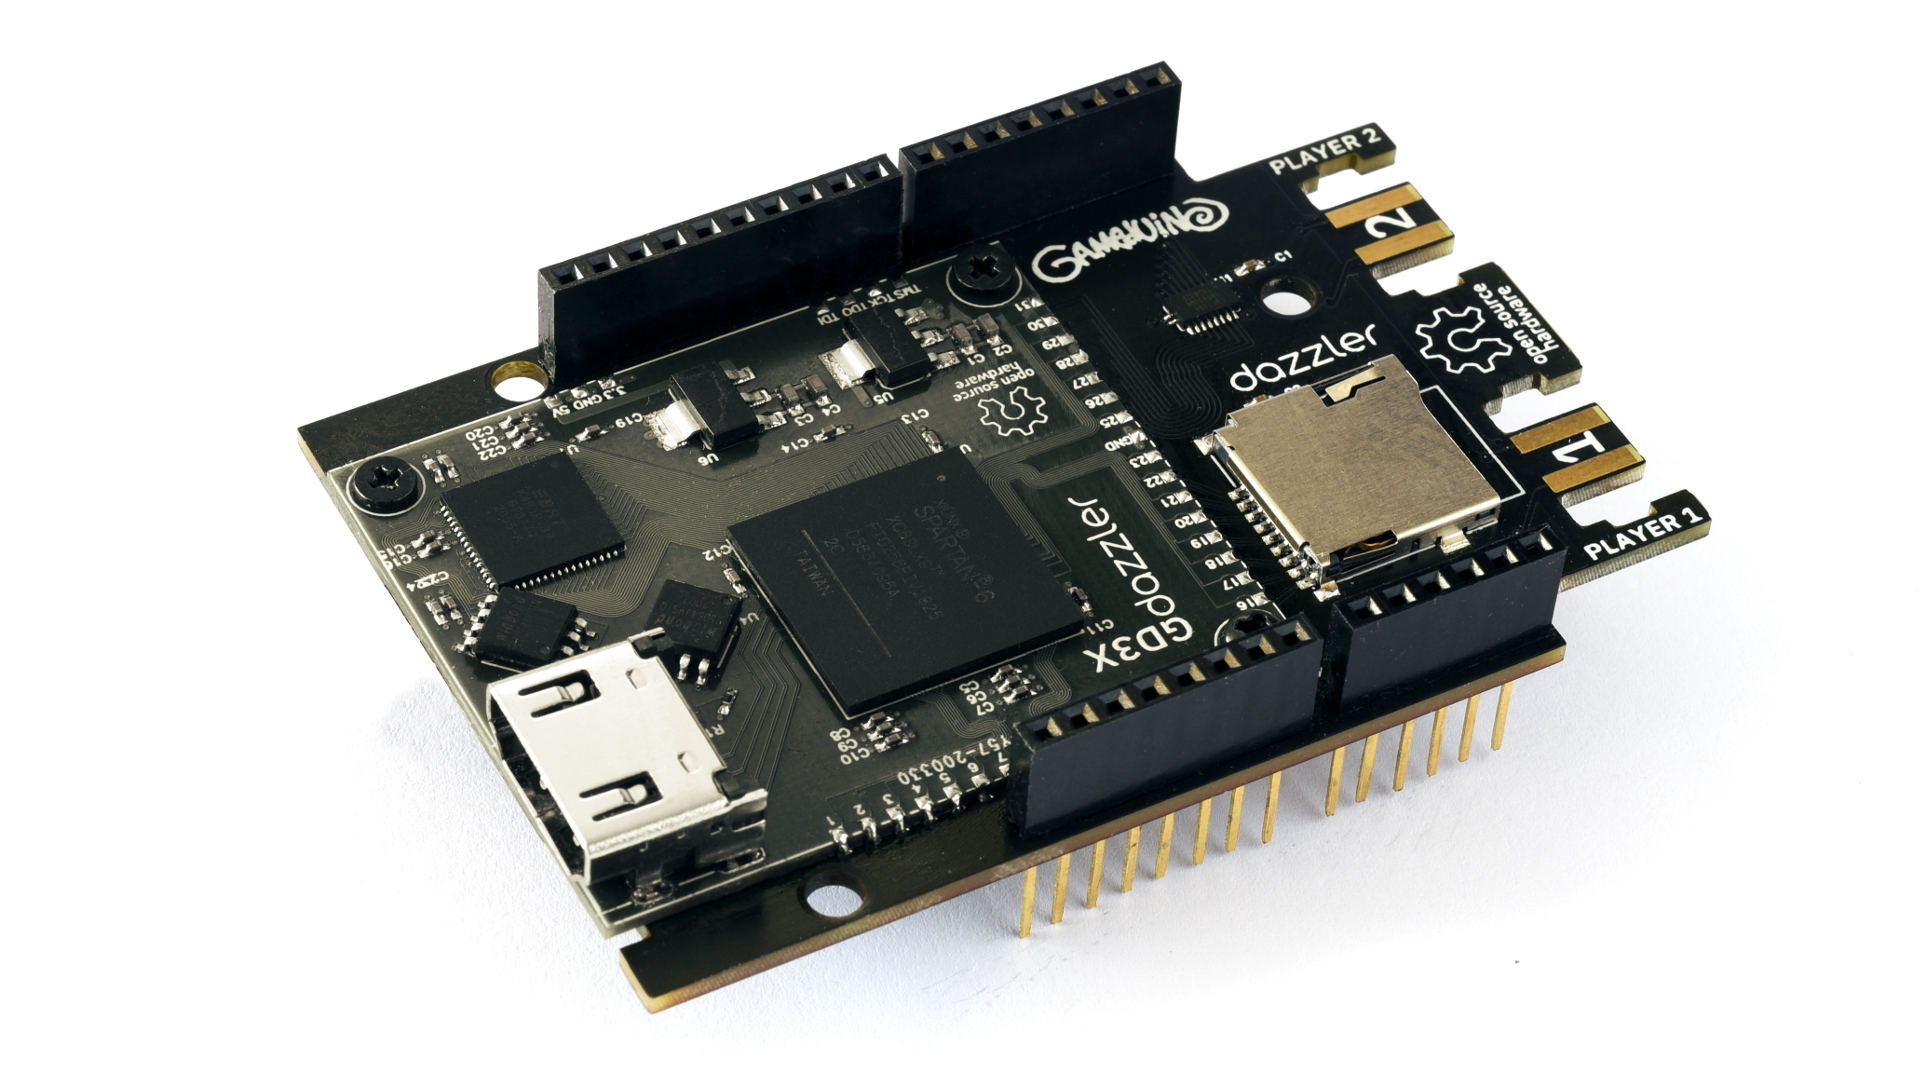
\includegraphics[width=1.00\textwidth]{img/gameduino-3x-dazzler/gameduino-3x-dazzler-main}
Last updated on \today
\end{center}
\tableofcontents

\newpage

\setlength{\parindent}{0mm}
\setlength{\parskip}{1mm}
\setstretch{1.4}

\section{Overview}

\png{img/gameduino-3x-dazzler/module}

The \device{} outputs HD picture and sound to any HDMI display.

It is available as a core module, and as an Arduino-compatible shield.

\subsection{Features}

The core module has the following features:

\begin{itemize}
\item Powerful BT815 embedded GPU with 24 bit color
\item HDMI encoding and system management handled by Xilinx Spartan-6 LX9 FPGA
\item 2 $\times$ 8 Megabyte flash
\item HDMI video output at 1280x720 @ 60 Hz (720p), audio output at 48 KHz
\item All features accessible via SPI interface
\item Single 5V supply; onboard regulation to 3.3V and 1.2V
\end{itemize}

\noindent
The shield adds:
\begin{itemize}
\item a level shifter so all inputs are 5V tolerant
\item a microSD card slot
\item 2 Wii Classic ports, both continuously scanned by the Dazzler
\item optional headers for standard serial and JTAG connectors
\end{itemize}

\png{img/gameduino-3x-dazzler/rot-0182}

\newpage
\section{Getting Started}

On power-up, the \dev{} displays a boot screen like this:

\pngw{img/gameduino-3x-dazzler/boot}{1.0}

The code on the left is the module's serial number. \index{serial number}
The center code is the firmware version. \index{firmware version}
On the right is the firmware build date.

\newpage
\section{Text mode}

\newpage
\section{Pinouts}

\subsection{Shield}
The Dazzler Shield follows the standard Arduino Uno pinout.

\gap
\begin{center}
\begin{tabular}{ccl}
\hline
GND	& power & Signal ground \\
5V	& power	& Main supply: 5-9V \\
\\
13	& in	& SPI SCK \\
12	& out	& SPI MISO \\
11	& in	& SPI MOSI \\
\\
10	& in	& DAZZLER SEL \\
9	& in	& SD SEL \\
8	& in	& GPU SEL \\
\\
2	& out	& INTERRUPT \\
1	& in 	& SERIAL IN \\
\hline
\end{tabular}
\end{center}
\gap

All other pins are pass-through.

\subsection{Module}

\pngw{img/gameduino-3x-dazzler/pinout}{1.0}

\newpage
\section{Internals}



\tikzstyle{block} = [draw, fill=white, rectangle, minimum height=40mm, minimum width=20mm]
\tikzstyle{sum} = [draw, fill=blue!20, circle, node distance=1cm]
\tikzstyle{input} = [coordinate]
\tikzstyle{output} = [coordinate]
\tikzstyle{pinstyle} = [pin edge={to-,thin,black}]


% The block diagram code is probably more verbose than necessary
\begin{center}
\begin{tikzpicture}[node distance=2cm,>=latex']
    % We start by placing the blocks
    \node [block] (FPGA) {FPGA};
\end{tikzpicture}
\end{center}

This is 

\newpage
\section{Specifications}\label{electrical-characteristics}

\subsection{DC characteristics}
\vspace{10 pt}
{\renewcommand{\arraystretch}{1.2}% for the vertical padding

\begin{tabularx}{\linewidth}{XC{40pt}C{40pt}C{40pt}C{40pt}}
& min & typ & max & units \\ \heavyline

All inputs signals & & & & \\
\hspace{10pt}low voltage & -0.5 & & 0.8 & V \\
\hspace{10pt}high voltage & 2.0 &   & 4.1 & V \\ \hline
Supply voltage        & 4.5 & 5.0 & 9.0 & V                   \\ \hline
Current consumption   & & 180 & & mA                   \\ \hline

\end{tabularx}}
\vspace{10 pt}

\subsection{AC characteristics}
\vspace{10 pt}

{\renewcommand{\arraystretch}{1.2}% for the vertical padding
\begin{tabularx}{\linewidth}{XC{40pt}C{40pt}C{40pt}C{40pt}}
& min & typ & max & units \\ \heavyline

SPI speed                     & & & 36 & Mbps   \index{speed!SPI}\\ \hline
Startup time & & & 270 & ms \\ \hline
Scanout frequency & & 74.25 $\pm$ 0.002\%  & & MHz  \\ \hline
Scanout frame rate & & 60.000 & & Hz  \\ \hline
\end{tabularx}}
\vspace{10 pt}

\subsection{Physical characteristics}
\vspace{10 pt}

{\renewcommand{\arraystretch}{1.2}% for the vertical padding
\begin{tabularx}{\linewidth}{XC{120pt}C{40pt}}
& & units \\ \heavyline

Dimensions (shield)           & 83 $\times$ 53 $\times$ 20 & mm   \index{dimensions}\\ \hline
Weight (shield)               & 32 & g   \index{weight}\\ \hline
Dimensions (module)           & 50 $\times$ 42 $\times$ 8.5 & mm   \index{dimensions}\\ \hline
Weight (module)               & 10 & g   \index{weight}\\ \hline

\end{tabularx}}
\vspace{10 pt}

\subsection{Module mechanical drawing}

All measurements are in mm.

The three mounting holes are designed for M2.5 screws, nuts and standoffs.

\begin{center}
\begin{tikzpicture}[scale=1.7]
\begin{tikzpicture}[scale=2]
\draw[color=blue, line width=.2mm] (0.000000mm,0.024549mm) -- (0.000000mm,5.651228mm) -- (0.025000mm,5.650000mm) -- (0.059306mm,5.651685mm) -- (0.093282mm,5.656725mm) -- (0.126600mm,5.665071mm) -- (0.158939mm,5.676642mm) -- (0.189989mm,5.691328mm) -- (0.219450mm,5.708986mm) -- (0.247038mm,5.729446mm) -- (0.272487mm,5.752513mm) -- (0.295554mm,5.777962mm) -- (0.316014mm,5.805550mm) -- (0.333672mm,5.835011mm) -- (0.348358mm,5.866061mm) -- (0.359929mm,5.898400mm) -- (0.368275mm,5.931718mm) -- (0.373315mm,5.965694mm) -- (0.375000mm,6.000000mm) -- (0.375000mm,6.000000mm) -- (0.373315mm,6.034306mm) -- (0.368275mm,6.068282mm) -- (0.359929mm,6.101600mm) -- (0.348358mm,6.133939mm) -- (0.333672mm,6.164989mm) -- (0.316014mm,6.194450mm) -- (0.295554mm,6.222038mm) -- (0.272487mm,6.247487mm) -- (0.247038mm,6.270554mm) -- (0.219450mm,6.291014mm) -- (0.189989mm,6.308672mm) -- (0.158939mm,6.323358mm) -- (0.126600mm,6.334929mm) -- (0.093282mm,6.343275mm) -- (0.059306mm,6.348315mm) -- (0.025000mm,6.350000mm) -- (0.000000mm,6.348772mm) -- (0.000000mm,7.651228mm) -- (0.025000mm,7.650000mm) -- (0.059306mm,7.651685mm) -- (0.093282mm,7.656725mm) -- (0.126600mm,7.665071mm) -- (0.158939mm,7.676642mm) -- (0.189989mm,7.691328mm) -- (0.219450mm,7.708986mm) -- (0.247038mm,7.729446mm) -- (0.272487mm,7.752513mm) -- (0.295554mm,7.777962mm) -- (0.316014mm,7.805550mm) -- (0.333672mm,7.835011mm) -- (0.348358mm,7.866061mm) -- (0.359929mm,7.898400mm) -- (0.368275mm,7.931718mm) -- (0.373315mm,7.965694mm) -- (0.375000mm,8.000000mm) -- (0.375000mm,8.000000mm) -- (0.373315mm,8.034306mm) -- (0.368275mm,8.068282mm) -- (0.359929mm,8.101600mm) -- (0.348358mm,8.133939mm) -- (0.333672mm,8.164989mm) -- (0.316014mm,8.194450mm) -- (0.295554mm,8.222038mm) -- (0.272487mm,8.247487mm) -- (0.247038mm,8.270554mm) -- (0.219450mm,8.291014mm) -- (0.189989mm,8.308672mm) -- (0.158939mm,8.323358mm) -- (0.126600mm,8.334929mm) -- (0.093282mm,8.343275mm) -- (0.059306mm,8.348315mm) -- (0.025000mm,8.350000mm) -- (0.000000mm,8.348772mm) -- (0.000000mm,9.651228mm) -- (0.025000mm,9.650000mm) -- (0.059306mm,9.651685mm) -- (0.093282mm,9.656725mm) -- (0.126600mm,9.665071mm) -- (0.158939mm,9.676642mm) -- (0.189989mm,9.691328mm) -- (0.219450mm,9.708986mm) -- (0.247038mm,9.729446mm) -- (0.272487mm,9.752513mm) -- (0.295554mm,9.777962mm) -- (0.316014mm,9.805550mm) -- (0.333672mm,9.835011mm) -- (0.348358mm,9.866061mm) -- (0.359929mm,9.898400mm) -- (0.368275mm,9.931718mm) -- (0.373315mm,9.965694mm) -- (0.375000mm,10.000000mm) -- (0.375000mm,10.000000mm) -- (0.373315mm,10.034306mm) -- (0.368275mm,10.068282mm) -- (0.359929mm,10.101600mm) -- (0.348358mm,10.133939mm) -- (0.333672mm,10.164989mm) -- (0.316014mm,10.194450mm) -- (0.295554mm,10.222038mm) -- (0.272487mm,10.247487mm) -- (0.247038mm,10.270554mm) -- (0.219450mm,10.291014mm) -- (0.189989mm,10.308672mm) -- (0.158939mm,10.323358mm) -- (0.126600mm,10.334929mm) -- (0.093282mm,10.343275mm) -- (0.059306mm,10.348315mm) -- (0.025000mm,10.350000mm) -- (0.000000mm,10.348772mm) -- (0.000000mm,11.651228mm) -- (0.025000mm,11.650000mm) -- (0.059306mm,11.651685mm) -- (0.093282mm,11.656725mm) -- (0.126600mm,11.665071mm) -- (0.158939mm,11.676642mm) -- (0.189989mm,11.691328mm) -- (0.219450mm,11.708986mm) -- (0.247038mm,11.729446mm) -- (0.272487mm,11.752513mm) -- (0.295554mm,11.777962mm) -- (0.316014mm,11.805550mm) -- (0.333672mm,11.835011mm) -- (0.348358mm,11.866061mm) -- (0.359929mm,11.898400mm) -- (0.368275mm,11.931718mm) -- (0.373315mm,11.965694mm) -- (0.375000mm,12.000000mm) -- (0.375000mm,12.000000mm) -- (0.373315mm,12.034306mm) -- (0.368275mm,12.068282mm) -- (0.359929mm,12.101600mm) -- (0.348358mm,12.133939mm) -- (0.333672mm,12.164989mm) -- (0.316014mm,12.194450mm) -- (0.295554mm,12.222038mm) -- (0.272487mm,12.247487mm) -- (0.247038mm,12.270554mm) -- (0.219450mm,12.291014mm) -- (0.189989mm,12.308672mm) -- (0.158939mm,12.323358mm) -- (0.126600mm,12.334929mm) -- (0.093282mm,12.343275mm) -- (0.059306mm,12.348315mm) -- (0.025000mm,12.350000mm) -- (0.000000mm,12.348772mm) -- (0.000000mm,13.651228mm) -- (0.025000mm,13.650000mm) -- (0.059306mm,13.651685mm) -- (0.093282mm,13.656725mm) -- (0.126600mm,13.665071mm) -- (0.158939mm,13.676642mm) -- (0.189989mm,13.691328mm) -- (0.219450mm,13.708986mm) -- (0.247038mm,13.729446mm) -- (0.272487mm,13.752513mm) -- (0.295554mm,13.777962mm) -- (0.316014mm,13.805550mm) -- (0.333672mm,13.835011mm) -- (0.348358mm,13.866061mm) -- (0.359929mm,13.898400mm) -- (0.368275mm,13.931718mm) -- (0.373315mm,13.965694mm) -- (0.375000mm,14.000000mm) -- (0.375000mm,14.000000mm) -- (0.373315mm,14.034306mm) -- (0.368275mm,14.068282mm) -- (0.359929mm,14.101600mm) -- (0.348358mm,14.133939mm) -- (0.333672mm,14.164989mm) -- (0.316014mm,14.194450mm) -- (0.295554mm,14.222038mm) -- (0.272487mm,14.247487mm) -- (0.247038mm,14.270554mm) -- (0.219450mm,14.291014mm) -- (0.189989mm,14.308672mm) -- (0.158939mm,14.323358mm) -- (0.126600mm,14.334929mm) -- (0.093282mm,14.343275mm) -- (0.059306mm,14.348315mm) -- (0.025000mm,14.350000mm) -- (0.000000mm,14.348772mm) -- (0.000000mm,15.651228mm) -- (0.025000mm,15.650000mm) -- (0.059306mm,15.651685mm) -- (0.093282mm,15.656725mm) -- (0.126600mm,15.665071mm) -- (0.158939mm,15.676642mm) -- (0.189989mm,15.691328mm) -- (0.219450mm,15.708986mm) -- (0.247038mm,15.729446mm) -- (0.272487mm,15.752513mm) -- (0.295554mm,15.777962mm) -- (0.316014mm,15.805550mm) -- (0.333672mm,15.835011mm) -- (0.348358mm,15.866061mm) -- (0.359929mm,15.898400mm) -- (0.368275mm,15.931718mm) -- (0.373315mm,15.965694mm) -- (0.375000mm,16.000000mm) -- (0.375000mm,16.000000mm) -- (0.373315mm,16.034306mm) -- (0.368275mm,16.068282mm) -- (0.359929mm,16.101600mm) -- (0.348358mm,16.133939mm) -- (0.333672mm,16.164989mm) -- (0.316014mm,16.194450mm) -- (0.295554mm,16.222038mm) -- (0.272487mm,16.247487mm) -- (0.247038mm,16.270554mm) -- (0.219450mm,16.291014mm) -- (0.189989mm,16.308672mm) -- (0.158939mm,16.323358mm) -- (0.126600mm,16.334929mm) -- (0.093282mm,16.343275mm) -- (0.059306mm,16.348315mm) -- (0.025000mm,16.350000mm) -- (0.000000mm,16.348772mm) -- (0.000000mm,17.651228mm) -- (0.025000mm,17.650000mm) -- (0.059306mm,17.651685mm) -- (0.093282mm,17.656725mm) -- (0.126600mm,17.665071mm) -- (0.158939mm,17.676642mm) -- (0.189989mm,17.691328mm) -- (0.219450mm,17.708986mm) -- (0.247038mm,17.729446mm) -- (0.272487mm,17.752513mm) -- (0.295554mm,17.777962mm) -- (0.316014mm,17.805550mm) -- (0.333672mm,17.835011mm) -- (0.348358mm,17.866061mm) -- (0.359929mm,17.898400mm) -- (0.368275mm,17.931718mm) -- (0.373315mm,17.965694mm) -- (0.375000mm,18.000000mm) -- (0.375000mm,18.000000mm) -- (0.373315mm,18.034306mm) -- (0.368275mm,18.068282mm) -- (0.359929mm,18.101600mm) -- (0.348358mm,18.133939mm) -- (0.333672mm,18.164989mm) -- (0.316014mm,18.194450mm) -- (0.295554mm,18.222038mm) -- (0.272487mm,18.247487mm) -- (0.247038mm,18.270554mm) -- (0.219450mm,18.291014mm) -- (0.189989mm,18.308672mm) -- (0.158939mm,18.323358mm) -- (0.126600mm,18.334929mm) -- (0.093282mm,18.343275mm) -- (0.059306mm,18.348315mm) -- (0.025000mm,18.350000mm) -- (0.000000mm,18.348772mm) -- (0.000000mm,19.651228mm) -- (0.025000mm,19.650000mm) -- (0.059306mm,19.651685mm) -- (0.093282mm,19.656725mm) -- (0.126600mm,19.665071mm) -- (0.158939mm,19.676642mm) -- (0.189989mm,19.691328mm) -- (0.219450mm,19.708986mm) -- (0.247038mm,19.729446mm) -- (0.272487mm,19.752513mm) -- (0.295554mm,19.777962mm) -- (0.316014mm,19.805550mm) -- (0.333672mm,19.835011mm) -- (0.348358mm,19.866061mm) -- (0.359929mm,19.898400mm) -- (0.368275mm,19.931718mm) -- (0.373315mm,19.965694mm) -- (0.375000mm,20.000000mm) -- (0.375000mm,20.000000mm) -- (0.373315mm,20.034306mm) -- (0.368275mm,20.068282mm) -- (0.359929mm,20.101600mm) -- (0.348358mm,20.133939mm) -- (0.333672mm,20.164989mm) -- (0.316014mm,20.194450mm) -- (0.295554mm,20.222038mm) -- (0.272487mm,20.247487mm) -- (0.247038mm,20.270554mm) -- (0.219450mm,20.291014mm) -- (0.189989mm,20.308672mm) -- (0.158939mm,20.323358mm) -- (0.126600mm,20.334929mm) -- (0.093282mm,20.343275mm) -- (0.059306mm,20.348315mm) -- (0.025000mm,20.350000mm) -- (0.000000mm,20.348772mm) -- (0.000000mm,21.651228mm) -- (0.025000mm,21.650000mm) -- (0.059306mm,21.651685mm) -- (0.093282mm,21.656725mm) -- (0.126600mm,21.665071mm) -- (0.158939mm,21.676642mm) -- (0.189989mm,21.691328mm) -- (0.219450mm,21.708986mm) -- (0.247038mm,21.729446mm) -- (0.272487mm,21.752513mm) -- (0.295554mm,21.777962mm) -- (0.316014mm,21.805550mm) -- (0.333672mm,21.835011mm) -- (0.348358mm,21.866061mm) -- (0.359929mm,21.898400mm) -- (0.368275mm,21.931718mm) -- (0.373315mm,21.965694mm) -- (0.375000mm,22.000000mm) -- (0.375000mm,22.000000mm) -- (0.373315mm,22.034306mm) -- (0.368275mm,22.068282mm) -- (0.359929mm,22.101600mm) -- (0.348358mm,22.133939mm) -- (0.333672mm,22.164989mm) -- (0.316014mm,22.194450mm) -- (0.295554mm,22.222038mm) -- (0.272487mm,22.247487mm) -- (0.247038mm,22.270554mm) -- (0.219450mm,22.291014mm) -- (0.189989mm,22.308672mm) -- (0.158939mm,22.323358mm) -- (0.126600mm,22.334929mm) -- (0.093282mm,22.343275mm) -- (0.059306mm,22.348315mm) -- (0.025000mm,22.350000mm) -- (0.000000mm,22.348772mm) -- (0.000000mm,23.651228mm) -- (0.025000mm,23.650000mm) -- (0.059306mm,23.651685mm) -- (0.093282mm,23.656725mm) -- (0.126600mm,23.665071mm) -- (0.158939mm,23.676642mm) -- (0.189989mm,23.691328mm) -- (0.219450mm,23.708986mm) -- (0.247038mm,23.729446mm) -- (0.272487mm,23.752513mm) -- (0.295554mm,23.777962mm) -- (0.316014mm,23.805550mm) -- (0.333672mm,23.835011mm) -- (0.348358mm,23.866061mm) -- (0.359929mm,23.898400mm) -- (0.368275mm,23.931718mm) -- (0.373315mm,23.965694mm) -- (0.375000mm,24.000000mm) -- (0.375000mm,24.000000mm) -- (0.373315mm,24.034306mm) -- (0.368275mm,24.068282mm) -- (0.359929mm,24.101600mm) -- (0.348358mm,24.133939mm) -- (0.333672mm,24.164989mm) -- (0.316014mm,24.194450mm) -- (0.295554mm,24.222038mm) -- (0.272487mm,24.247487mm) -- (0.247038mm,24.270554mm) -- (0.219450mm,24.291014mm) -- (0.189989mm,24.308672mm) -- (0.158939mm,24.323358mm) -- (0.126600mm,24.334929mm) -- (0.093282mm,24.343275mm) -- (0.059306mm,24.348315mm) -- (0.025000mm,24.350000mm) -- (0.000000mm,24.348772mm) -- (0.000000mm,25.651228mm) -- (0.025000mm,25.650000mm) -- (0.059306mm,25.651685mm) -- (0.093282mm,25.656725mm) -- (0.126600mm,25.665071mm) -- (0.158939mm,25.676642mm) -- (0.189989mm,25.691328mm) -- (0.219450mm,25.708986mm) -- (0.247038mm,25.729446mm) -- (0.272487mm,25.752513mm) -- (0.295554mm,25.777962mm) -- (0.316014mm,25.805550mm) -- (0.333672mm,25.835011mm) -- (0.348358mm,25.866061mm) -- (0.359929mm,25.898400mm) -- (0.368275mm,25.931718mm) -- (0.373315mm,25.965694mm) -- (0.375000mm,26.000000mm) -- (0.375000mm,26.000000mm) -- (0.373315mm,26.034306mm) -- (0.368275mm,26.068282mm) -- (0.359929mm,26.101600mm) -- (0.348358mm,26.133939mm) -- (0.333672mm,26.164989mm) -- (0.316014mm,26.194450mm) -- (0.295554mm,26.222038mm) -- (0.272487mm,26.247487mm) -- (0.247038mm,26.270554mm) -- (0.219450mm,26.291014mm) -- (0.189989mm,26.308672mm) -- (0.158939mm,26.323358mm) -- (0.126600mm,26.334929mm) -- (0.093282mm,26.343275mm) -- (0.059306mm,26.348315mm) -- (0.025000mm,26.350000mm) -- (0.000000mm,26.348772mm) -- (0.000000mm,27.651228mm) -- (0.025000mm,27.650000mm) -- (0.059306mm,27.651685mm) -- (0.093282mm,27.656725mm) -- (0.126600mm,27.665071mm) -- (0.158939mm,27.676642mm) -- (0.189989mm,27.691328mm) -- (0.219450mm,27.708986mm) -- (0.247038mm,27.729446mm) -- (0.272487mm,27.752513mm) -- (0.295554mm,27.777962mm) -- (0.316014mm,27.805550mm) -- (0.333672mm,27.835011mm) -- (0.348358mm,27.866061mm) -- (0.359929mm,27.898400mm) -- (0.368275mm,27.931718mm) -- (0.373315mm,27.965694mm) -- (0.375000mm,28.000000mm) -- (0.375000mm,28.000000mm) -- (0.373315mm,28.034306mm) -- (0.368275mm,28.068282mm) -- (0.359929mm,28.101600mm) -- (0.348358mm,28.133939mm) -- (0.333672mm,28.164989mm) -- (0.316014mm,28.194450mm) -- (0.295554mm,28.222038mm) -- (0.272487mm,28.247487mm) -- (0.247038mm,28.270554mm) -- (0.219450mm,28.291014mm) -- (0.189989mm,28.308672mm) -- (0.158939mm,28.323358mm) -- (0.126600mm,28.334929mm) -- (0.093282mm,28.343275mm) -- (0.059306mm,28.348315mm) -- (0.025000mm,28.350000mm) -- (0.000000mm,28.348772mm) -- (0.000000mm,29.651228mm) -- (0.025000mm,29.650000mm) -- (0.059306mm,29.651685mm) -- (0.093282mm,29.656725mm) -- (0.126600mm,29.665071mm) -- (0.158939mm,29.676642mm) -- (0.189989mm,29.691328mm) -- (0.219450mm,29.708986mm) -- (0.247038mm,29.729446mm) -- (0.272487mm,29.752513mm) -- (0.295554mm,29.777962mm) -- (0.316014mm,29.805550mm) -- (0.333672mm,29.835011mm) -- (0.348358mm,29.866061mm) -- (0.359929mm,29.898400mm) -- (0.368275mm,29.931718mm) -- (0.373315mm,29.965694mm) -- (0.375000mm,30.000000mm) -- (0.375000mm,30.000000mm) -- (0.373315mm,30.034306mm) -- (0.368275mm,30.068282mm) -- (0.359929mm,30.101600mm) -- (0.348358mm,30.133939mm) -- (0.333672mm,30.164989mm) -- (0.316014mm,30.194450mm) -- (0.295554mm,30.222038mm) -- (0.272487mm,30.247487mm) -- (0.247038mm,30.270554mm) -- (0.219450mm,30.291014mm) -- (0.189989mm,30.308672mm) -- (0.158939mm,30.323358mm) -- (0.126600mm,30.334929mm) -- (0.093282mm,30.343275mm) -- (0.059306mm,30.348315mm) -- (0.025000mm,30.350000mm) -- (0.000000mm,30.348772mm) -- (0.000000mm,31.651228mm) -- (0.025000mm,31.650000mm) -- (0.059306mm,31.651685mm) -- (0.093282mm,31.656725mm) -- (0.126600mm,31.665071mm) -- (0.158939mm,31.676642mm) -- (0.189989mm,31.691328mm) -- (0.219450mm,31.708986mm) -- (0.247038mm,31.729446mm) -- (0.272487mm,31.752513mm) -- (0.295554mm,31.777962mm) -- (0.316014mm,31.805550mm) -- (0.333672mm,31.835011mm) -- (0.348358mm,31.866061mm) -- (0.359929mm,31.898400mm) -- (0.368275mm,31.931718mm) -- (0.373315mm,31.965694mm) -- (0.375000mm,32.000000mm) -- (0.373315mm,32.034306mm) -- (0.368275mm,32.068282mm) -- (0.359929mm,32.101600mm) -- (0.348358mm,32.133939mm) -- (0.333672mm,32.164989mm) -- (0.316014mm,32.194450mm) -- (0.295554mm,32.222038mm) -- (0.272487mm,32.247487mm) -- (0.247038mm,32.270554mm) -- (0.219450mm,32.291014mm) -- (0.189989mm,32.308672mm) -- (0.158939mm,32.323358mm) -- (0.126600mm,32.334929mm) -- (0.093282mm,32.343275mm) -- (0.059306mm,32.348315mm) -- (0.025000mm,32.350000mm) -- (0.000000mm,32.348772mm) -- (0.000000mm,33.651228mm) -- (0.025000mm,33.650000mm) -- (0.059306mm,33.651685mm) -- (0.093282mm,33.656725mm) -- (0.126600mm,33.665071mm) -- (0.158939mm,33.676642mm) -- (0.189989mm,33.691328mm) -- (0.219450mm,33.708986mm) -- (0.247038mm,33.729446mm) -- (0.272487mm,33.752513mm) -- (0.295554mm,33.777962mm) -- (0.316014mm,33.805550mm) -- (0.333672mm,33.835011mm) -- (0.348358mm,33.866061mm) -- (0.359929mm,33.898400mm) -- (0.368275mm,33.931718mm) -- (0.373315mm,33.965694mm) -- (0.375000mm,34.000000mm) -- (0.373315mm,34.034306mm) -- (0.368275mm,34.068282mm) -- (0.359929mm,34.101600mm) -- (0.348358mm,34.133939mm) -- (0.333672mm,34.164989mm) -- (0.316014mm,34.194450mm) -- (0.295554mm,34.222038mm) -- (0.272487mm,34.247487mm) -- (0.247038mm,34.270554mm) -- (0.219450mm,34.291014mm) -- (0.189989mm,34.308672mm) -- (0.158939mm,34.323358mm) -- (0.126600mm,34.334929mm) -- (0.093282mm,34.343275mm) -- (0.059306mm,34.348315mm) -- (0.025000mm,34.350000mm) -- (0.000000mm,34.348772mm) -- (0.000000mm,35.651228mm) -- (0.025000mm,35.650000mm) -- (0.059306mm,35.651685mm) -- (0.093282mm,35.656725mm) -- (0.126600mm,35.665071mm) -- (0.158939mm,35.676642mm) -- (0.189989mm,35.691328mm) -- (0.219450mm,35.708986mm) -- (0.247038mm,35.729446mm) -- (0.272487mm,35.752513mm) -- (0.295554mm,35.777962mm) -- (0.316014mm,35.805550mm) -- (0.333672mm,35.835011mm) -- (0.348358mm,35.866061mm) -- (0.359929mm,35.898400mm) -- (0.368275mm,35.931718mm) -- (0.373315mm,35.965694mm) -- (0.375000mm,36.000000mm) -- (0.373315mm,36.034306mm) -- (0.368275mm,36.068282mm) -- (0.359929mm,36.101600mm) -- (0.348358mm,36.133939mm) -- (0.333672mm,36.164989mm) -- (0.316014mm,36.194450mm) -- (0.295554mm,36.222038mm) -- (0.272487mm,36.247487mm) -- (0.247038mm,36.270554mm) -- (0.219450mm,36.291014mm) -- (0.189989mm,36.308672mm) -- (0.158939mm,36.323358mm) -- (0.126600mm,36.334929mm) -- (0.093282mm,36.343275mm) -- (0.059306mm,36.348315mm) -- (0.025000mm,36.350000mm) -- (0.000000mm,36.348772mm) -- (0.000000mm,41.975451mm) -- (0.001150mm,41.998850mm) -- (0.024549mm,42.000000mm) -- (5.651228mm,42.000000mm) -- (5.650000mm,41.975000mm) -- (5.651685mm,41.940694mm) -- (5.656725mm,41.906718mm) -- (5.665071mm,41.873400mm) -- (5.676642mm,41.841061mm) -- (5.691328mm,41.810011mm) -- (5.708986mm,41.780550mm) -- (5.729446mm,41.752962mm) -- (5.752513mm,41.727513mm) -- (5.777962mm,41.704446mm) -- (5.805550mm,41.683986mm) -- (5.835011mm,41.666328mm) -- (5.866061mm,41.651642mm) -- (5.898400mm,41.640071mm) -- (5.931718mm,41.631725mm) -- (5.965694mm,41.626685mm) -- (6.000000mm,41.625000mm) -- (6.034306mm,41.626685mm) -- (6.068282mm,41.631725mm) -- (6.101600mm,41.640071mm) -- (6.133939mm,41.651642mm) -- (6.164989mm,41.666328mm) -- (6.194450mm,41.683986mm) -- (6.222038mm,41.704446mm) -- (6.247487mm,41.727513mm) -- (6.270554mm,41.752962mm) -- (6.291014mm,41.780550mm) -- (6.308672mm,41.810011mm) -- (6.323358mm,41.841061mm) -- (6.334929mm,41.873400mm) -- (6.343275mm,41.906718mm) -- (6.348315mm,41.940694mm) -- (6.350000mm,41.975000mm) -- (6.348772mm,42.000000mm) -- (7.651228mm,42.000000mm) -- (7.650000mm,41.975000mm) -- (7.651685mm,41.940694mm) -- (7.656725mm,41.906718mm) -- (7.665071mm,41.873400mm) -- (7.676642mm,41.841061mm) -- (7.691328mm,41.810011mm) -- (7.708986mm,41.780550mm) -- (7.729446mm,41.752962mm) -- (7.752513mm,41.727513mm) -- (7.777962mm,41.704446mm) -- (7.805550mm,41.683986mm) -- (7.835011mm,41.666328mm) -- (7.866061mm,41.651642mm) -- (7.898400mm,41.640071mm) -- (7.931718mm,41.631725mm) -- (7.965694mm,41.626685mm) -- (8.000000mm,41.625000mm) -- (8.034306mm,41.626685mm) -- (8.068282mm,41.631725mm) -- (8.101600mm,41.640071mm) -- (8.133939mm,41.651642mm) -- (8.164989mm,41.666328mm) -- (8.194450mm,41.683986mm) -- (8.222038mm,41.704446mm) -- (8.247487mm,41.727513mm) -- (8.270554mm,41.752962mm) -- (8.291014mm,41.780550mm) -- (8.308672mm,41.810011mm) -- (8.323358mm,41.841061mm) -- (8.334929mm,41.873400mm) -- (8.343275mm,41.906718mm) -- (8.348315mm,41.940694mm) -- (8.350000mm,41.975000mm) -- (8.348772mm,42.000000mm) -- (9.651228mm,42.000000mm) -- (9.650000mm,41.975000mm) -- (9.651685mm,41.940694mm) -- (9.656725mm,41.906718mm) -- (9.665071mm,41.873400mm) -- (9.676642mm,41.841061mm) -- (9.691328mm,41.810011mm) -- (9.708986mm,41.780550mm) -- (9.729446mm,41.752962mm) -- (9.752513mm,41.727513mm) -- (9.777962mm,41.704446mm) -- (9.805550mm,41.683986mm) -- (9.835011mm,41.666328mm) -- (9.866061mm,41.651642mm) -- (9.898400mm,41.640071mm) -- (9.931718mm,41.631725mm) -- (9.965694mm,41.626685mm) -- (10.000000mm,41.625000mm) -- (10.034306mm,41.626685mm) -- (10.068282mm,41.631725mm) -- (10.101600mm,41.640071mm) -- (10.133939mm,41.651642mm) -- (10.164989mm,41.666328mm) -- (10.194450mm,41.683986mm) -- (10.222038mm,41.704446mm) -- (10.247487mm,41.727513mm) -- (10.270554mm,41.752962mm) -- (10.291014mm,41.780550mm) -- (10.308672mm,41.810011mm) -- (10.323358mm,41.841061mm) -- (10.334929mm,41.873400mm) -- (10.343275mm,41.906718mm) -- (10.348315mm,41.940694mm) -- (10.350000mm,41.975000mm) -- (10.348772mm,42.000000mm) -- (11.651228mm,42.000000mm) -- (11.650000mm,41.975000mm) -- (11.651685mm,41.940694mm) -- (11.656725mm,41.906718mm) -- (11.665071mm,41.873400mm) -- (11.676642mm,41.841061mm) -- (11.691328mm,41.810011mm) -- (11.708986mm,41.780550mm) -- (11.729446mm,41.752962mm) -- (11.752513mm,41.727513mm) -- (11.777962mm,41.704446mm) -- (11.805550mm,41.683986mm) -- (11.835011mm,41.666328mm) -- (11.866061mm,41.651642mm) -- (11.898400mm,41.640071mm) -- (11.931718mm,41.631725mm) -- (11.965694mm,41.626685mm) -- (12.000000mm,41.625000mm) -- (12.034306mm,41.626685mm) -- (12.068282mm,41.631725mm) -- (12.101600mm,41.640071mm) -- (12.133939mm,41.651642mm) -- (12.164989mm,41.666328mm) -- (12.194450mm,41.683986mm) -- (12.222038mm,41.704446mm) -- (12.247487mm,41.727513mm) -- (12.270554mm,41.752962mm) -- (12.291014mm,41.780550mm) -- (12.308672mm,41.810011mm) -- (12.323358mm,41.841061mm) -- (12.334929mm,41.873400mm) -- (12.343275mm,41.906718mm) -- (12.348315mm,41.940694mm) -- (12.350000mm,41.975000mm) -- (12.348772mm,42.000000mm) -- (13.651228mm,42.000000mm) -- (13.650000mm,41.975000mm) -- (13.651685mm,41.940694mm) -- (13.656725mm,41.906718mm) -- (13.665071mm,41.873400mm) -- (13.676642mm,41.841061mm) -- (13.691328mm,41.810011mm) -- (13.708986mm,41.780550mm) -- (13.729446mm,41.752962mm) -- (13.752513mm,41.727513mm) -- (13.777962mm,41.704446mm) -- (13.805550mm,41.683986mm) -- (13.835011mm,41.666328mm) -- (13.866061mm,41.651642mm) -- (13.898400mm,41.640071mm) -- (13.931718mm,41.631725mm) -- (13.965694mm,41.626685mm) -- (14.000000mm,41.625000mm) -- (14.034306mm,41.626685mm) -- (14.068282mm,41.631725mm) -- (14.101600mm,41.640071mm) -- (14.133939mm,41.651642mm) -- (14.164989mm,41.666328mm) -- (14.194450mm,41.683986mm) -- (14.222038mm,41.704446mm) -- (14.247487mm,41.727513mm) -- (14.270554mm,41.752962mm) -- (14.291014mm,41.780550mm) -- (14.308672mm,41.810011mm) -- (14.323358mm,41.841061mm) -- (14.334929mm,41.873400mm) -- (14.343275mm,41.906718mm) -- (14.348315mm,41.940694mm) -- (14.350000mm,41.975000mm) -- (14.348772mm,42.000000mm) -- (15.651228mm,42.000000mm) -- (15.650000mm,41.975000mm) -- (15.651685mm,41.940694mm) -- (15.656725mm,41.906718mm) -- (15.665071mm,41.873400mm) -- (15.676642mm,41.841061mm) -- (15.691328mm,41.810011mm) -- (15.708986mm,41.780550mm) -- (15.729446mm,41.752962mm) -- (15.752513mm,41.727513mm) -- (15.777962mm,41.704446mm) -- (15.805550mm,41.683986mm) -- (15.835011mm,41.666328mm) -- (15.866061mm,41.651642mm) -- (15.898400mm,41.640071mm) -- (15.931718mm,41.631725mm) -- (15.965694mm,41.626685mm) -- (16.000000mm,41.625000mm) -- (16.034306mm,41.626685mm) -- (16.068282mm,41.631725mm) -- (16.101600mm,41.640071mm) -- (16.133939mm,41.651642mm) -- (16.164989mm,41.666328mm) -- (16.194450mm,41.683986mm) -- (16.222038mm,41.704446mm) -- (16.247487mm,41.727513mm) -- (16.270554mm,41.752962mm) -- (16.291014mm,41.780550mm) -- (16.308672mm,41.810011mm) -- (16.323358mm,41.841061mm) -- (16.334929mm,41.873400mm) -- (16.343275mm,41.906718mm) -- (16.348315mm,41.940694mm) -- (16.350000mm,41.975000mm) -- (16.348772mm,42.000000mm) -- (17.651228mm,42.000000mm) -- (17.650000mm,41.975000mm) -- (17.651685mm,41.940694mm) -- (17.656725mm,41.906718mm) -- (17.665071mm,41.873400mm) -- (17.676642mm,41.841061mm) -- (17.691328mm,41.810011mm) -- (17.708986mm,41.780550mm) -- (17.729446mm,41.752962mm) -- (17.752513mm,41.727513mm) -- (17.777962mm,41.704446mm) -- (17.805550mm,41.683986mm) -- (17.835011mm,41.666328mm) -- (17.866061mm,41.651642mm) -- (17.898400mm,41.640071mm) -- (17.931718mm,41.631725mm) -- (17.965694mm,41.626685mm) -- (18.000000mm,41.625000mm) -- (18.034306mm,41.626685mm) -- (18.068282mm,41.631725mm) -- (18.101600mm,41.640071mm) -- (18.133939mm,41.651642mm) -- (18.164989mm,41.666328mm) -- (18.194450mm,41.683986mm) -- (18.222038mm,41.704446mm) -- (18.247487mm,41.727513mm) -- (18.270554mm,41.752962mm) -- (18.291014mm,41.780550mm) -- (18.308672mm,41.810011mm) -- (18.323358mm,41.841061mm) -- (18.334929mm,41.873400mm) -- (18.343275mm,41.906718mm) -- (18.348315mm,41.940694mm) -- (18.350000mm,41.975000mm) -- (18.348772mm,42.000000mm) -- (19.651228mm,42.000000mm) -- (19.650000mm,41.975000mm) -- (19.651685mm,41.940694mm) -- (19.656725mm,41.906718mm) -- (19.665071mm,41.873400mm) -- (19.676642mm,41.841061mm) -- (19.691328mm,41.810011mm) -- (19.708986mm,41.780550mm) -- (19.729446mm,41.752962mm) -- (19.752513mm,41.727513mm) -- (19.777962mm,41.704446mm) -- (19.805550mm,41.683986mm) -- (19.835011mm,41.666328mm) -- (19.866061mm,41.651642mm) -- (19.898400mm,41.640071mm) -- (19.931718mm,41.631725mm) -- (19.965694mm,41.626685mm) -- (20.000000mm,41.625000mm) -- (20.034306mm,41.626685mm) -- (20.068282mm,41.631725mm) -- (20.101600mm,41.640071mm) -- (20.133939mm,41.651642mm) -- (20.164989mm,41.666328mm) -- (20.194450mm,41.683986mm) -- (20.222038mm,41.704446mm) -- (20.247487mm,41.727513mm) -- (20.270554mm,41.752962mm) -- (20.291014mm,41.780550mm) -- (20.308672mm,41.810011mm) -- (20.323358mm,41.841061mm) -- (20.334929mm,41.873400mm) -- (20.343275mm,41.906718mm) -- (20.348315mm,41.940694mm) -- (20.350000mm,41.975000mm) -- (20.348772mm,42.000000mm) -- (21.651228mm,42.000000mm) -- (21.650000mm,41.975000mm) -- (21.651685mm,41.940694mm) -- (21.656725mm,41.906718mm) -- (21.665071mm,41.873400mm) -- (21.676642mm,41.841061mm) -- (21.691328mm,41.810011mm) -- (21.708986mm,41.780550mm) -- (21.729446mm,41.752962mm) -- (21.752513mm,41.727513mm) -- (21.777962mm,41.704446mm) -- (21.805550mm,41.683986mm) -- (21.835011mm,41.666328mm) -- (21.866061mm,41.651642mm) -- (21.898400mm,41.640071mm) -- (21.931718mm,41.631725mm) -- (21.965694mm,41.626685mm) -- (22.000000mm,41.625000mm) -- (22.034306mm,41.626685mm) -- (22.068282mm,41.631725mm) -- (22.101600mm,41.640071mm) -- (22.133939mm,41.651642mm) -- (22.164989mm,41.666328mm) -- (22.194450mm,41.683986mm) -- (22.222038mm,41.704446mm) -- (22.247487mm,41.727513mm) -- (22.270554mm,41.752962mm) -- (22.291014mm,41.780550mm) -- (22.308672mm,41.810011mm) -- (22.323358mm,41.841061mm) -- (22.334929mm,41.873400mm) -- (22.343275mm,41.906718mm) -- (22.348315mm,41.940694mm) -- (22.350000mm,41.975000mm) -- (22.348772mm,42.000000mm) -- (23.651228mm,42.000000mm) -- (23.650000mm,41.975000mm) -- (23.651685mm,41.940694mm) -- (23.656725mm,41.906718mm) -- (23.665071mm,41.873400mm) -- (23.676642mm,41.841061mm) -- (23.691328mm,41.810011mm) -- (23.708986mm,41.780550mm) -- (23.729446mm,41.752962mm) -- (23.752513mm,41.727513mm) -- (23.777962mm,41.704446mm) -- (23.805550mm,41.683986mm) -- (23.835011mm,41.666328mm) -- (23.866061mm,41.651642mm) -- (23.898400mm,41.640071mm) -- (23.931718mm,41.631725mm) -- (23.965694mm,41.626685mm) -- (24.000000mm,41.625000mm) -- (24.034306mm,41.626685mm) -- (24.068282mm,41.631725mm) -- (24.101600mm,41.640071mm) -- (24.133939mm,41.651642mm) -- (24.164989mm,41.666328mm) -- (24.194450mm,41.683986mm) -- (24.222038mm,41.704446mm) -- (24.247487mm,41.727513mm) -- (24.270554mm,41.752962mm) -- (24.291014mm,41.780550mm) -- (24.308672mm,41.810011mm) -- (24.323358mm,41.841061mm) -- (24.334929mm,41.873400mm) -- (24.343275mm,41.906718mm) -- (24.348315mm,41.940694mm) -- (24.350000mm,41.975000mm) -- (24.348772mm,42.000000mm) -- (25.651228mm,42.000000mm) -- (25.650000mm,41.975000mm) -- (25.651685mm,41.940694mm) -- (25.656725mm,41.906718mm) -- (25.665071mm,41.873400mm) -- (25.676642mm,41.841061mm) -- (25.691328mm,41.810011mm) -- (25.708986mm,41.780550mm) -- (25.729446mm,41.752962mm) -- (25.752513mm,41.727513mm) -- (25.777962mm,41.704446mm) -- (25.805550mm,41.683986mm) -- (25.835011mm,41.666328mm) -- (25.866061mm,41.651642mm) -- (25.898400mm,41.640071mm) -- (25.931718mm,41.631725mm) -- (25.965694mm,41.626685mm) -- (26.000000mm,41.625000mm) -- (26.034306mm,41.626685mm) -- (26.068282mm,41.631725mm) -- (26.101600mm,41.640071mm) -- (26.133939mm,41.651642mm) -- (26.164989mm,41.666328mm) -- (26.194450mm,41.683986mm) -- (26.222038mm,41.704446mm) -- (26.247487mm,41.727513mm) -- (26.270554mm,41.752962mm) -- (26.291014mm,41.780550mm) -- (26.308672mm,41.810011mm) -- (26.323358mm,41.841061mm) -- (26.334929mm,41.873400mm) -- (26.343275mm,41.906718mm) -- (26.348315mm,41.940694mm) -- (26.350000mm,41.975000mm) -- (26.348772mm,42.000000mm) -- (27.651228mm,42.000000mm) -- (27.650000mm,41.975000mm) -- (27.651685mm,41.940694mm) -- (27.656725mm,41.906718mm) -- (27.665071mm,41.873400mm) -- (27.676642mm,41.841061mm) -- (27.691328mm,41.810011mm) -- (27.708986mm,41.780550mm) -- (27.729446mm,41.752962mm) -- (27.752513mm,41.727513mm) -- (27.777962mm,41.704446mm) -- (27.805550mm,41.683986mm) -- (27.835011mm,41.666328mm) -- (27.866061mm,41.651642mm) -- (27.898400mm,41.640071mm) -- (27.931718mm,41.631725mm) -- (27.965694mm,41.626685mm) -- (28.000000mm,41.625000mm) -- (28.034306mm,41.626685mm) -- (28.068282mm,41.631725mm) -- (28.101600mm,41.640071mm) -- (28.133939mm,41.651642mm) -- (28.164989mm,41.666328mm) -- (28.194450mm,41.683986mm) -- (28.222038mm,41.704446mm) -- (28.247487mm,41.727513mm) -- (28.270554mm,41.752962mm) -- (28.291014mm,41.780550mm) -- (28.308672mm,41.810011mm) -- (28.323358mm,41.841061mm) -- (28.334929mm,41.873400mm) -- (28.343275mm,41.906718mm) -- (28.348315mm,41.940694mm) -- (28.350000mm,41.975000mm) -- (28.348772mm,42.000000mm) -- (29.651228mm,42.000000mm) -- (29.650000mm,41.975000mm) -- (29.651685mm,41.940694mm) -- (29.656725mm,41.906718mm) -- (29.665071mm,41.873400mm) -- (29.676642mm,41.841061mm) -- (29.691328mm,41.810011mm) -- (29.708986mm,41.780550mm) -- (29.729446mm,41.752962mm) -- (29.752513mm,41.727513mm) -- (29.777962mm,41.704446mm) -- (29.805550mm,41.683986mm) -- (29.835011mm,41.666328mm) -- (29.866061mm,41.651642mm) -- (29.898400mm,41.640071mm) -- (29.931718mm,41.631725mm) -- (29.965694mm,41.626685mm) -- (30.000000mm,41.625000mm) -- (30.034306mm,41.626685mm) -- (30.068282mm,41.631725mm) -- (30.101600mm,41.640071mm) -- (30.133939mm,41.651642mm) -- (30.164989mm,41.666328mm) -- (30.194450mm,41.683986mm) -- (30.222038mm,41.704446mm) -- (30.247487mm,41.727513mm) -- (30.270554mm,41.752962mm) -- (30.291014mm,41.780550mm) -- (30.308672mm,41.810011mm) -- (30.323358mm,41.841061mm) -- (30.334929mm,41.873400mm) -- (30.343275mm,41.906718mm) -- (30.348315mm,41.940694mm) -- (30.350000mm,41.975000mm) -- (30.348772mm,42.000000mm) -- (31.651228mm,42.000000mm) -- (31.650000mm,41.975000mm) -- (31.651685mm,41.940694mm) -- (31.656725mm,41.906718mm) -- (31.665071mm,41.873400mm) -- (31.676642mm,41.841061mm) -- (31.691328mm,41.810011mm) -- (31.708986mm,41.780550mm) -- (31.729446mm,41.752962mm) -- (31.752513mm,41.727513mm) -- (31.777962mm,41.704446mm) -- (31.805550mm,41.683986mm) -- (31.835011mm,41.666328mm) -- (31.866061mm,41.651642mm) -- (31.898400mm,41.640071mm) -- (31.931718mm,41.631725mm) -- (31.965694mm,41.626685mm) -- (32.000000mm,41.625000mm) -- (32.034306mm,41.626685mm) -- (32.068282mm,41.631725mm) -- (32.101600mm,41.640071mm) -- (32.133939mm,41.651642mm) -- (32.164989mm,41.666328mm) -- (32.194450mm,41.683986mm) -- (32.222038mm,41.704446mm) -- (32.247487mm,41.727513mm) -- (32.270554mm,41.752962mm) -- (32.291014mm,41.780550mm) -- (32.308672mm,41.810011mm) -- (32.323358mm,41.841061mm) -- (32.334929mm,41.873400mm) -- (32.343275mm,41.906718mm) -- (32.348315mm,41.940694mm) -- (32.350000mm,41.975000mm) -- (32.348772mm,42.000000mm) -- (33.651228mm,42.000000mm) -- (33.650000mm,41.975000mm) -- (33.651685mm,41.940694mm) -- (33.656725mm,41.906718mm) -- (33.665071mm,41.873400mm) -- (33.676642mm,41.841061mm) -- (33.691328mm,41.810011mm) -- (33.708986mm,41.780550mm) -- (33.729446mm,41.752962mm) -- (33.752513mm,41.727513mm) -- (33.777962mm,41.704446mm) -- (33.805550mm,41.683986mm) -- (33.835011mm,41.666328mm) -- (33.866061mm,41.651642mm) -- (33.898400mm,41.640071mm) -- (33.931718mm,41.631725mm) -- (33.965694mm,41.626685mm) -- (34.000000mm,41.625000mm) -- (34.034306mm,41.626685mm) -- (34.068282mm,41.631725mm) -- (34.101600mm,41.640071mm) -- (34.133939mm,41.651642mm) -- (34.164989mm,41.666328mm) -- (34.194450mm,41.683986mm) -- (34.222038mm,41.704446mm) -- (34.247487mm,41.727513mm) -- (34.270554mm,41.752962mm) -- (34.291014mm,41.780550mm) -- (34.308672mm,41.810011mm) -- (34.323358mm,41.841061mm) -- (34.334929mm,41.873400mm) -- (34.343275mm,41.906718mm) -- (34.348315mm,41.940694mm) -- (34.350000mm,41.975000mm) -- (34.348772mm,42.000000mm) -- (49.975451mm,42.000000mm) -- (49.998850mm,41.998850mm) -- (50.000000mm,41.975451mm) -- (50.000000mm,0.024549mm) -- (49.998850mm,0.001150mm) -- (49.975451mm,0.000000mm) -- (34.348772mm,0.000000mm) -- (34.350000mm,0.025000mm) -- (34.350000mm,0.025000mm) -- (34.348315mm,0.059306mm) -- (34.343275mm,0.093282mm) -- (34.334929mm,0.126600mm) -- (34.323358mm,0.158939mm) -- (34.308672mm,0.189989mm) -- (34.291014mm,0.219450mm) -- (34.270554mm,0.247038mm) -- (34.247487mm,0.272487mm) -- (34.222038mm,0.295554mm) -- (34.194450mm,0.316014mm) -- (34.164989mm,0.333672mm) -- (34.133939mm,0.348358mm) -- (34.101600mm,0.359929mm) -- (34.068282mm,0.368275mm) -- (34.034306mm,0.373315mm) -- (34.000000mm,0.375000mm) -- (33.965694mm,0.373315mm) -- (33.931718mm,0.368275mm) -- (33.898400mm,0.359929mm) -- (33.866061mm,0.348358mm) -- (33.835011mm,0.333672mm) -- (33.805550mm,0.316014mm) -- (33.777962mm,0.295554mm) -- (33.752513mm,0.272487mm) -- (33.729446mm,0.247038mm) -- (33.708986mm,0.219450mm) -- (33.691328mm,0.189989mm) -- (33.676642mm,0.158939mm) -- (33.665071mm,0.126600mm) -- (33.656725mm,0.093282mm) -- (33.651685mm,0.059306mm) -- (33.650000mm,0.025000mm) -- (33.651228mm,0.000000mm) -- (32.348772mm,0.000000mm) -- (32.350000mm,0.025000mm) -- (32.350000mm,0.025000mm) -- (32.348315mm,0.059306mm) -- (32.343275mm,0.093282mm) -- (32.334929mm,0.126600mm) -- (32.323358mm,0.158939mm) -- (32.308672mm,0.189989mm) -- (32.291014mm,0.219450mm) -- (32.270554mm,0.247038mm) -- (32.247487mm,0.272487mm) -- (32.222038mm,0.295554mm) -- (32.194450mm,0.316014mm) -- (32.164989mm,0.333672mm) -- (32.133939mm,0.348358mm) -- (32.101600mm,0.359929mm) -- (32.068282mm,0.368275mm) -- (32.034306mm,0.373315mm) -- (32.000000mm,0.375000mm) -- (31.965694mm,0.373315mm) -- (31.931718mm,0.368275mm) -- (31.898400mm,0.359929mm) -- (31.866061mm,0.348358mm) -- (31.835011mm,0.333672mm) -- (31.805550mm,0.316014mm) -- (31.777962mm,0.295554mm) -- (31.752513mm,0.272487mm) -- (31.729446mm,0.247038mm) -- (31.708986mm,0.219450mm) -- (31.691328mm,0.189989mm) -- (31.676642mm,0.158939mm) -- (31.665071mm,0.126600mm) -- (31.656725mm,0.093282mm) -- (31.651685mm,0.059306mm) -- (31.650000mm,0.025000mm) -- (31.651228mm,0.000000mm) -- (30.348772mm,0.000000mm) -- (30.350000mm,0.025000mm) -- (30.350000mm,0.025000mm) -- (30.348315mm,0.059306mm) -- (30.343275mm,0.093282mm) -- (30.334929mm,0.126600mm) -- (30.323358mm,0.158939mm) -- (30.308672mm,0.189989mm) -- (30.291014mm,0.219450mm) -- (30.270554mm,0.247038mm) -- (30.247487mm,0.272487mm) -- (30.222038mm,0.295554mm) -- (30.194450mm,0.316014mm) -- (30.164989mm,0.333672mm) -- (30.133939mm,0.348358mm) -- (30.101600mm,0.359929mm) -- (30.068282mm,0.368275mm) -- (30.034306mm,0.373315mm) -- (30.000000mm,0.375000mm) -- (29.965694mm,0.373315mm) -- (29.931718mm,0.368275mm) -- (29.898400mm,0.359929mm) -- (29.866061mm,0.348358mm) -- (29.835011mm,0.333672mm) -- (29.805550mm,0.316014mm) -- (29.777962mm,0.295554mm) -- (29.752513mm,0.272487mm) -- (29.729446mm,0.247038mm) -- (29.708986mm,0.219450mm) -- (29.691328mm,0.189989mm) -- (29.676642mm,0.158939mm) -- (29.665071mm,0.126600mm) -- (29.656725mm,0.093282mm) -- (29.651685mm,0.059306mm) -- (29.650000mm,0.025000mm) -- (29.651228mm,0.000000mm) -- (26.348772mm,0.000000mm) -- (26.350000mm,0.025000mm) -- (26.350000mm,0.025000mm) -- (26.348315mm,0.059306mm) -- (26.343275mm,0.093282mm) -- (26.334929mm,0.126600mm) -- (26.323358mm,0.158939mm) -- (26.308672mm,0.189989mm) -- (26.291014mm,0.219450mm) -- (26.270554mm,0.247038mm) -- (26.247487mm,0.272487mm) -- (26.222038mm,0.295554mm) -- (26.194450mm,0.316014mm) -- (26.164989mm,0.333672mm) -- (26.133939mm,0.348358mm) -- (26.101600mm,0.359929mm) -- (26.068282mm,0.368275mm) -- (26.034306mm,0.373315mm) -- (26.000000mm,0.375000mm) -- (25.965694mm,0.373315mm) -- (25.931718mm,0.368275mm) -- (25.898400mm,0.359929mm) -- (25.866061mm,0.348358mm) -- (25.835011mm,0.333672mm) -- (25.805550mm,0.316014mm) -- (25.777962mm,0.295554mm) -- (25.752513mm,0.272487mm) -- (25.729446mm,0.247038mm) -- (25.708986mm,0.219450mm) -- (25.691328mm,0.189989mm) -- (25.676642mm,0.158939mm) -- (25.665071mm,0.126600mm) -- (25.656725mm,0.093282mm) -- (25.651685mm,0.059306mm) -- (25.650000mm,0.025000mm) -- (25.651228mm,0.000000mm) -- (24.348772mm,0.000000mm) -- (24.350000mm,0.025000mm) -- (24.350000mm,0.025000mm) -- (24.348315mm,0.059306mm) -- (24.343275mm,0.093282mm) -- (24.334929mm,0.126600mm) -- (24.323358mm,0.158939mm) -- (24.308672mm,0.189989mm) -- (24.291014mm,0.219450mm) -- (24.270554mm,0.247038mm) -- (24.247487mm,0.272487mm) -- (24.222038mm,0.295554mm) -- (24.194450mm,0.316014mm) -- (24.164989mm,0.333672mm) -- (24.133939mm,0.348358mm) -- (24.101600mm,0.359929mm) -- (24.068282mm,0.368275mm) -- (24.034306mm,0.373315mm) -- (24.000000mm,0.375000mm) -- (23.965694mm,0.373315mm) -- (23.931718mm,0.368275mm) -- (23.898400mm,0.359929mm) -- (23.866061mm,0.348358mm) -- (23.835011mm,0.333672mm) -- (23.805550mm,0.316014mm) -- (23.777962mm,0.295554mm) -- (23.752513mm,0.272487mm) -- (23.729446mm,0.247038mm) -- (23.708986mm,0.219450mm) -- (23.691328mm,0.189989mm) -- (23.676642mm,0.158939mm) -- (23.665071mm,0.126600mm) -- (23.656725mm,0.093282mm) -- (23.651685mm,0.059306mm) -- (23.650000mm,0.025000mm) -- (23.651228mm,0.000000mm) -- (22.348772mm,0.000000mm) -- (22.350000mm,0.025000mm) -- (22.350000mm,0.025000mm) -- (22.348315mm,0.059306mm) -- (22.343275mm,0.093282mm) -- (22.334929mm,0.126600mm) -- (22.323358mm,0.158939mm) -- (22.308672mm,0.189989mm) -- (22.291014mm,0.219450mm) -- (22.270554mm,0.247038mm) -- (22.247487mm,0.272487mm) -- (22.222038mm,0.295554mm) -- (22.194450mm,0.316014mm) -- (22.164989mm,0.333672mm) -- (22.133939mm,0.348358mm) -- (22.101600mm,0.359929mm) -- (22.068282mm,0.368275mm) -- (22.034306mm,0.373315mm) -- (22.000000mm,0.375000mm) -- (21.965694mm,0.373315mm) -- (21.931718mm,0.368275mm) -- (21.898400mm,0.359929mm) -- (21.866061mm,0.348358mm) -- (21.835011mm,0.333672mm) -- (21.805550mm,0.316014mm) -- (21.777962mm,0.295554mm) -- (21.752513mm,0.272487mm) -- (21.729446mm,0.247038mm) -- (21.708986mm,0.219450mm) -- (21.691328mm,0.189989mm) -- (21.676642mm,0.158939mm) -- (21.665071mm,0.126600mm) -- (21.656725mm,0.093282mm) -- (21.651685mm,0.059306mm) -- (21.650000mm,0.025000mm) -- (21.651228mm,0.000000mm) -- (20.348772mm,0.000000mm) -- (20.350000mm,0.025000mm) -- (20.350000mm,0.025000mm) -- (20.348315mm,0.059306mm) -- (20.343275mm,0.093282mm) -- (20.334929mm,0.126600mm) -- (20.323358mm,0.158939mm) -- (20.308672mm,0.189989mm) -- (20.291014mm,0.219450mm) -- (20.270554mm,0.247038mm) -- (20.247487mm,0.272487mm) -- (20.222038mm,0.295554mm) -- (20.194450mm,0.316014mm) -- (20.164989mm,0.333672mm) -- (20.133939mm,0.348358mm) -- (20.101600mm,0.359929mm) -- (20.068282mm,0.368275mm) -- (20.034306mm,0.373315mm) -- (20.000000mm,0.375000mm) -- (19.965694mm,0.373315mm) -- (19.931718mm,0.368275mm) -- (19.898400mm,0.359929mm) -- (19.866061mm,0.348358mm) -- (19.835011mm,0.333672mm) -- (19.805550mm,0.316014mm) -- (19.777962mm,0.295554mm) -- (19.752513mm,0.272487mm) -- (19.729446mm,0.247038mm) -- (19.708986mm,0.219450mm) -- (19.691328mm,0.189989mm) -- (19.676642mm,0.158939mm) -- (19.665071mm,0.126600mm) -- (19.656725mm,0.093282mm) -- (19.651685mm,0.059306mm) -- (19.650000mm,0.025000mm) -- (19.651228mm,0.000000mm) -- (16.348772mm,0.000000mm) -- (16.350000mm,0.025000mm) -- (16.350000mm,0.025000mm) -- (16.348315mm,0.059306mm) -- (16.343275mm,0.093282mm) -- (16.334929mm,0.126600mm) -- (16.323358mm,0.158939mm) -- (16.308672mm,0.189989mm) -- (16.291014mm,0.219450mm) -- (16.270554mm,0.247038mm) -- (16.247487mm,0.272487mm) -- (16.222038mm,0.295554mm) -- (16.194450mm,0.316014mm) -- (16.164989mm,0.333672mm) -- (16.133939mm,0.348358mm) -- (16.101600mm,0.359929mm) -- (16.068282mm,0.368275mm) -- (16.034306mm,0.373315mm) -- (16.000000mm,0.375000mm) -- (15.965694mm,0.373315mm) -- (15.931718mm,0.368275mm) -- (15.898400mm,0.359929mm) -- (15.866061mm,0.348358mm) -- (15.835011mm,0.333672mm) -- (15.805550mm,0.316014mm) -- (15.777962mm,0.295554mm) -- (15.752513mm,0.272487mm) -- (15.729446mm,0.247038mm) -- (15.708986mm,0.219450mm) -- (15.691328mm,0.189989mm) -- (15.676642mm,0.158939mm) -- (15.665071mm,0.126600mm) -- (15.656725mm,0.093282mm) -- (15.651685mm,0.059306mm) -- (15.650000mm,0.025000mm) -- (15.651228mm,0.000000mm) -- (14.348772mm,0.000000mm) -- (14.350000mm,0.025000mm) -- (14.350000mm,0.025000mm) -- (14.348315mm,0.059306mm) -- (14.343275mm,0.093282mm) -- (14.334929mm,0.126600mm) -- (14.323358mm,0.158939mm) -- (14.308672mm,0.189989mm) -- (14.291014mm,0.219450mm) -- (14.270554mm,0.247038mm) -- (14.247487mm,0.272487mm) -- (14.222038mm,0.295554mm) -- (14.194450mm,0.316014mm) -- (14.164989mm,0.333672mm) -- (14.133939mm,0.348358mm) -- (14.101600mm,0.359929mm) -- (14.068282mm,0.368275mm) -- (14.034306mm,0.373315mm) -- (14.000000mm,0.375000mm) -- (13.965694mm,0.373315mm) -- (13.931718mm,0.368275mm) -- (13.898400mm,0.359929mm) -- (13.866061mm,0.348358mm) -- (13.835011mm,0.333672mm) -- (13.805550mm,0.316014mm) -- (13.777962mm,0.295554mm) -- (13.752513mm,0.272487mm) -- (13.729446mm,0.247038mm) -- (13.708986mm,0.219450mm) -- (13.691328mm,0.189989mm) -- (13.676642mm,0.158939mm) -- (13.665071mm,0.126600mm) -- (13.656725mm,0.093282mm) -- (13.651685mm,0.059306mm) -- (13.650000mm,0.025000mm) -- (13.651228mm,0.000000mm) -- (12.348772mm,0.000000mm) -- (12.350000mm,0.025000mm) -- (12.350000mm,0.025000mm) -- (12.348315mm,0.059306mm) -- (12.343275mm,0.093282mm) -- (12.334929mm,0.126600mm) -- (12.323358mm,0.158939mm) -- (12.308672mm,0.189989mm) -- (12.291014mm,0.219450mm) -- (12.270554mm,0.247038mm) -- (12.247487mm,0.272487mm) -- (12.222038mm,0.295554mm) -- (12.194450mm,0.316014mm) -- (12.164989mm,0.333672mm) -- (12.133939mm,0.348358mm) -- (12.101600mm,0.359929mm) -- (12.068282mm,0.368275mm) -- (12.034306mm,0.373315mm) -- (12.000000mm,0.375000mm) -- (11.965694mm,0.373315mm) -- (11.931718mm,0.368275mm) -- (11.898400mm,0.359929mm) -- (11.866061mm,0.348358mm) -- (11.835011mm,0.333672mm) -- (11.805550mm,0.316014mm) -- (11.777962mm,0.295554mm) -- (11.752513mm,0.272487mm) -- (11.729446mm,0.247038mm) -- (11.708986mm,0.219450mm) -- (11.691328mm,0.189989mm) -- (11.676642mm,0.158939mm) -- (11.665071mm,0.126600mm) -- (11.656725mm,0.093282mm) -- (11.651685mm,0.059306mm) -- (11.650000mm,0.025000mm) -- (11.651228mm,0.000000mm) -- (10.348772mm,0.000000mm) -- (10.350000mm,0.025000mm) -- (10.350000mm,0.025000mm) -- (10.348315mm,0.059306mm) -- (10.343275mm,0.093282mm) -- (10.334929mm,0.126600mm) -- (10.323358mm,0.158939mm) -- (10.308672mm,0.189989mm) -- (10.291014mm,0.219450mm) -- (10.270554mm,0.247038mm) -- (10.247487mm,0.272487mm) -- (10.222038mm,0.295554mm) -- (10.194450mm,0.316014mm) -- (10.164989mm,0.333672mm) -- (10.133939mm,0.348358mm) -- (10.101600mm,0.359929mm) -- (10.068282mm,0.368275mm) -- (10.034306mm,0.373315mm) -- (10.000000mm,0.375000mm) -- (9.965694mm,0.373315mm) -- (9.931718mm,0.368275mm) -- (9.898400mm,0.359929mm) -- (9.866061mm,0.348358mm) -- (9.835011mm,0.333672mm) -- (9.805550mm,0.316014mm) -- (9.777962mm,0.295554mm) -- (9.752513mm,0.272487mm) -- (9.729446mm,0.247038mm) -- (9.708986mm,0.219450mm) -- (9.691328mm,0.189989mm) -- (9.676642mm,0.158939mm) -- (9.665071mm,0.126600mm) -- (9.656725mm,0.093282mm) -- (9.651685mm,0.059306mm) -- (9.650000mm,0.025000mm) -- (9.651228mm,0.000000mm) -- (8.348772mm,0.000000mm) -- (8.350000mm,0.025000mm) -- (8.350000mm,0.025000mm) -- (8.348315mm,0.059306mm) -- (8.343275mm,0.093282mm) -- (8.334929mm,0.126600mm) -- (8.323358mm,0.158939mm) -- (8.308672mm,0.189989mm) -- (8.291014mm,0.219450mm) -- (8.270554mm,0.247038mm) -- (8.247487mm,0.272487mm) -- (8.222038mm,0.295554mm) -- (8.194450mm,0.316014mm) -- (8.164989mm,0.333672mm) -- (8.133939mm,0.348358mm) -- (8.101600mm,0.359929mm) -- (8.068282mm,0.368275mm) -- (8.034306mm,0.373315mm) -- (8.000000mm,0.375000mm) -- (7.965694mm,0.373315mm) -- (7.931718mm,0.368275mm) -- (7.898400mm,0.359929mm) -- (7.866061mm,0.348358mm) -- (7.835011mm,0.333672mm) -- (7.805550mm,0.316014mm) -- (7.777962mm,0.295554mm) -- (7.752513mm,0.272487mm) -- (7.729446mm,0.247038mm) -- (7.708986mm,0.219450mm) -- (7.691328mm,0.189989mm) -- (7.676642mm,0.158939mm) -- (7.665071mm,0.126600mm) -- (7.656725mm,0.093282mm) -- (7.651685mm,0.059306mm) -- (7.650000mm,0.025000mm) -- (7.651228mm,0.000000mm) -- (0.024549mm,0.000000mm) -- (0.001150mm,0.001150mm) -- (0.000000mm,0.024549mm);
\draw[color=blue, line width=.2mm] (48.450000mm,2.800000mm) -- (48.450000mm,2.800000mm) -- (48.443981mm,2.922521mm) -- (48.425982mm,3.043863mm) -- (48.396175mm,3.162856mm) -- (48.354849mm,3.278354mm) -- (48.302402mm,3.389246mm) -- (48.239337mm,3.494463mm) -- (48.166263mm,3.592992mm) -- (48.083883mm,3.683883mm) -- (47.992992mm,3.766263mm) -- (47.894463mm,3.839337mm) -- (47.789246mm,3.902402mm) -- (47.678354mm,3.954849mm) -- (47.562856mm,3.996175mm) -- (47.443863mm,4.025982mm) -- (47.322521mm,4.043981mm) -- (47.200000mm,4.050000mm) -- (47.077479mm,4.043981mm) -- (46.956137mm,4.025982mm) -- (46.837144mm,3.996175mm) -- (46.721646mm,3.954849mm) -- (46.610754mm,3.902402mm) -- (46.505537mm,3.839337mm) -- (46.407008mm,3.766263mm) -- (46.316117mm,3.683883mm) -- (46.233737mm,3.592992mm) -- (46.160663mm,3.494463mm) -- (46.097598mm,3.389246mm) -- (46.045151mm,3.278354mm) -- (46.003825mm,3.162856mm) -- (45.974018mm,3.043863mm) -- (45.956019mm,2.922521mm) -- (45.950000mm,2.800000mm) -- (45.956019mm,2.677479mm) -- (45.974018mm,2.556137mm) -- (46.003825mm,2.437144mm) -- (46.045151mm,2.321646mm) -- (46.097598mm,2.210754mm) -- (46.160663mm,2.105537mm) -- (46.233737mm,2.007008mm) -- (46.316117mm,1.916117mm) -- (46.407008mm,1.833737mm) -- (46.505537mm,1.760663mm) -- (46.610754mm,1.697598mm) -- (46.721646mm,1.645151mm) -- (46.837144mm,1.603825mm) -- (46.956137mm,1.574018mm) -- (47.077479mm,1.556019mm) -- (47.200000mm,1.550000mm) -- (47.322521mm,1.556019mm) -- (47.443863mm,1.574018mm) -- (47.562856mm,1.603825mm) -- (47.678354mm,1.645151mm) -- (47.789246mm,1.697598mm) -- (47.894463mm,1.760663mm) -- (47.992992mm,1.833737mm) -- (48.083883mm,1.916117mm) -- (48.166263mm,2.007008mm) -- (48.239337mm,2.105537mm) -- (48.302402mm,2.210754mm) -- (48.354849mm,2.321646mm) -- (48.396175mm,2.437144mm) -- (48.425982mm,2.556137mm) -- (48.443981mm,2.677479mm) -- (48.450000mm,2.800000mm);
\draw[color=blue, line width=.2mm] (4.050000mm,2.800000mm) -- (4.050000mm,2.800000mm) -- (4.043981mm,2.922521mm) -- (4.025982mm,3.043863mm) -- (3.996175mm,3.162856mm) -- (3.954849mm,3.278354mm) -- (3.902402mm,3.389246mm) -- (3.839337mm,3.494463mm) -- (3.766263mm,3.592992mm) -- (3.683883mm,3.683883mm) -- (3.592992mm,3.766263mm) -- (3.494463mm,3.839337mm) -- (3.389246mm,3.902402mm) -- (3.278354mm,3.954849mm) -- (3.162856mm,3.996175mm) -- (3.043863mm,4.025982mm) -- (2.922521mm,4.043981mm) -- (2.800000mm,4.050000mm) -- (2.677479mm,4.043981mm) -- (2.556137mm,4.025982mm) -- (2.437144mm,3.996175mm) -- (2.321646mm,3.954849mm) -- (2.210754mm,3.902402mm) -- (2.105537mm,3.839337mm) -- (2.007008mm,3.766263mm) -- (1.916117mm,3.683883mm) -- (1.833737mm,3.592992mm) -- (1.760663mm,3.494463mm) -- (1.697598mm,3.389246mm) -- (1.645151mm,3.278354mm) -- (1.603825mm,3.162856mm) -- (1.574018mm,3.043863mm) -- (1.556019mm,2.922521mm) -- (1.550000mm,2.800000mm) -- (1.556019mm,2.677479mm) -- (1.574018mm,2.556137mm) -- (1.603825mm,2.437144mm) -- (1.645151mm,2.321646mm) -- (1.697598mm,2.210754mm) -- (1.760663mm,2.105537mm) -- (1.833737mm,2.007008mm) -- (1.916117mm,1.916117mm) -- (2.007008mm,1.833737mm) -- (2.105537mm,1.760663mm) -- (2.210754mm,1.697598mm) -- (2.321646mm,1.645151mm) -- (2.437144mm,1.603825mm) -- (2.556137mm,1.574018mm) -- (2.677479mm,1.556019mm) -- (2.800000mm,1.550000mm) -- (2.922521mm,1.556019mm) -- (3.043863mm,1.574018mm) -- (3.162856mm,1.603825mm) -- (3.278354mm,1.645151mm) -- (3.389246mm,1.697598mm) -- (3.494463mm,1.760663mm) -- (3.592992mm,1.833737mm) -- (3.683883mm,1.916117mm) -- (3.766263mm,2.007008mm) -- (3.839337mm,2.105537mm) -- (3.902402mm,2.210754mm) -- (3.954849mm,2.321646mm) -- (3.996175mm,2.437144mm) -- (4.025982mm,2.556137mm) -- (4.043981mm,2.677479mm) -- (4.050000mm,2.800000mm);
\draw[color=blue, line width=.2mm] (4.050000mm,39.200000mm) -- (4.050000mm,39.200000mm) -- (4.043981mm,39.322521mm) -- (4.025982mm,39.443863mm) -- (3.996175mm,39.562856mm) -- (3.954849mm,39.678354mm) -- (3.902402mm,39.789246mm) -- (3.839337mm,39.894463mm) -- (3.766263mm,39.992992mm) -- (3.683883mm,40.083883mm) -- (3.592992mm,40.166263mm) -- (3.494463mm,40.239337mm) -- (3.389246mm,40.302402mm) -- (3.278354mm,40.354849mm) -- (3.162856mm,40.396175mm) -- (3.043863mm,40.425982mm) -- (2.922521mm,40.443981mm) -- (2.800000mm,40.450000mm) -- (2.677479mm,40.443981mm) -- (2.556137mm,40.425982mm) -- (2.437144mm,40.396175mm) -- (2.321646mm,40.354849mm) -- (2.210754mm,40.302402mm) -- (2.105537mm,40.239337mm) -- (2.007008mm,40.166263mm) -- (1.916117mm,40.083883mm) -- (1.833737mm,39.992992mm) -- (1.760663mm,39.894463mm) -- (1.697598mm,39.789246mm) -- (1.645151mm,39.678354mm) -- (1.603825mm,39.562856mm) -- (1.574018mm,39.443863mm) -- (1.556019mm,39.322521mm) -- (1.550000mm,39.200000mm) -- (1.556019mm,39.077479mm) -- (1.574018mm,38.956137mm) -- (1.603825mm,38.837144mm) -- (1.645151mm,38.721646mm) -- (1.697598mm,38.610754mm) -- (1.760663mm,38.505537mm) -- (1.833737mm,38.407008mm) -- (1.916117mm,38.316117mm) -- (2.007008mm,38.233737mm) -- (2.105537mm,38.160663mm) -- (2.210754mm,38.097598mm) -- (2.321646mm,38.045151mm) -- (2.437144mm,38.003825mm) -- (2.556137mm,37.974018mm) -- (2.677479mm,37.956019mm) -- (2.800000mm,37.950000mm) -- (2.922521mm,37.956019mm) -- (3.043863mm,37.974018mm) -- (3.162856mm,38.003825mm) -- (3.278354mm,38.045151mm) -- (3.389246mm,38.097598mm) -- (3.494463mm,38.160663mm) -- (3.592992mm,38.233737mm) -- (3.683883mm,38.316117mm) -- (3.766263mm,38.407008mm) -- (3.839337mm,38.505537mm) -- (3.902402mm,38.610754mm) -- (3.954849mm,38.721646mm) -- (3.996175mm,38.837144mm) -- (4.025982mm,38.956137mm) -- (4.043981mm,39.077479mm) -- (4.050000mm,39.200000mm);
\end{tikzpicture}

    \coordinate (A) at (0,5);
    \coordinate (B) at (5,5);
    \dimline {(A)}{(B)}{50};
    \coordinate (C) at (5.8,4.2);
    \coordinate (D) at (5.8,0);
    \dimline {(C)}{(D)}{42};

    \coordinate (E) at (0,-0.7);
    \coordinate (F) at (.28,-0.7);
    \coordinate (G) at (4.72,-0.7);
    \coordinate (H) at (5,-0.7);
    \dimline [label style={below=0.5ex,font=\small}] {(F)}{(E)}{2.8};
    \dimline {(G)}{(F)}{44.4};
    \dimline [label style={below=0.5ex,font=\small}]{(H)}{(G)}{2.8};

    \coordinate (I) at (-0.7,0);
    \coordinate (J) at (-0.7,.28);
    \coordinate (K) at (-0.7,3.92);
    \coordinate (L) at (-0.7,4.20);
    \dimline [label style={above=0.5ex,font=\small}] {(I)}{(J)}{2.8};
    \dimline {(J)}{(K)}{36.4};
    \dimline [label style={above=0.5ex,font=\small}]{(K)}{(L)}{2.8};

    \dimline  [label style={above=0.5ex,font=\scriptsize},line style={arrows=dimline reverse-dimline reverse}]
    {(.28-.125,1.3)}{(.28+.125,1.3)}{$\diameter$ 2.5};
\end{tikzpicture}
\end{center}

\newpage
\section{Troubleshooting}

\gap
\begin{tabular}{|l|l|}
\hline
No monitor output after power-up     & $\bullet$ Check HDMI cable and port \\
                                     & $\bullet$ Confirm 5V power present \\
                                     & $\bullet$ Return for replacement \\
\hline
No audio output                      & $\bullet$ Confirm the display has audio output \\
                                     & $\bullet$ Check the display's mute and volume settings \\
\hline
\end{tabular}
\gap

\section{Support information}

Technical and product support is available at
\href{mailto:jamesb@excamera.com}{jamesb@excamera.com}

\device{} is built and maintained by
\href{https://excamera.com}{Excamera Labs}.


\newpage
\raggedright
\addcontentsline{toc}{section}{Index}
\renewcommand{\indexname}{Index}
\printindex

\end{document}
